% ============================================================
% Capítulo II — Propagación de una onda plana. Interferencias
% Traducción de "Théorie mathématique de la lumière" (1889), cap. II
% Original: §§40-61, páginas impresas 48-75
% ============================================================
\chapter{Propagación de una onda plana. Interferencias}
\label{cap:ondaplana}

\section{Caso particular del movimiento por ondas planas}

\noindent\textbf{40. Caso particular del movimiento por ondas planas.} —
Supongamos que las componentes $\xi,\eta,\zeta$ de
los desplazamientos, que en general son funciones de $x,y,z,t$, dependan
solo de $z$ y de $t$. Si se considera un plano perpendicular al eje $z$,
los desplazamientos de todas las moléculas de ese plano tendrán, en el
mismo instante $t$, el mismo valor, puesto que el $z$ de todos los puntos
del plano es el mismo. Ese plano es el plano de la onda.

En el caso de los movimientos transversales, la función isótropa $\Theta$
es idénticamente nula; ahora bien, puesto que en el movimiento que
consideramos $\xi,\eta,\zeta$ no dependen ni de $x$ ni de $y$, se tiene
$d\xi/dx=0$, $d\eta/dy=0$; y, por consiguiente, la condición $\Theta=0$ se
reduce a $d\zeta/dz=0$.

La componente $\zeta$ del desplazamiento es, pues, una constante; si la
suponemos nula, el desplazamiento de las moléculas del medio elástico
tiene lugar en el plano de la onda, lo que justifica la denominación de
movimientos transversales dada a los movimientos para los que se tiene
$\Theta=0$.

Los movimientos que hemos llamado movimientos longitudinales están
caracterizados por las identidades siguientes (§35):
\[
u=\frac{d\eta}{dz}-\frac{d\zeta}{dy}=0,\qquad
v=\frac{d\zeta}{dx}-\frac{d\xi}{dz}=0,\qquad
w=\frac{d\xi}{dy}-\frac{d\eta}{dx}=0.
\]
En el caso de las ondas planas estas condiciones se reducen a
$d\eta/dz=0$, $d\xi/dz=0$.

En el mismo instante $t$, las componentes $\xi$ y $\eta$ de los
desplazamientos de todas las moléculas son, pues, las mismas; si las
suponemos nulas, el desplazamiento de las moléculas tiene lugar según una
perpendicular al plano de la onda; por eso hemos llamado movimientos
longitudinales a los movimientos que satisfacen las condiciones
anteriores.

\noindent\textbf{41.} Las ecuaciones (39) de los movimientos transversales
en los cuerpos isótropos se simplifican en el caso de la propagación por
ondas planas; no dependiendo las cantidades $\xi,\eta,\zeta$ ni de $x$ ni
de $y$, se tiene, para el movimiento de la molécula en el plano de la
onda,
\[
-\rho\,\frac{d^2\xi}{dt^2} = 2\mu\,\frac{d^2\xi}{dz^2},\qquad
-\rho\,\frac{d^2\eta}{dt^2} = 2\mu\,\frac{d^2\eta}{dz^2}.
\]
Si ponemos
\[
V=\sqrt{-\frac{2\mu}{\rho}},
\]
estas ecuaciones se convierten en
\[
\frac{d^2\xi}{dt^2} = V^2\frac{d^2\xi}{dz^2},\qquad
\frac{d^2\eta}{dt^2} = V^2\frac{d^2\eta}{dz^2}.
\]
Integrando la primera, obtenemos
\[
\xi = F(z-Vt) + F'(z+Vt),
\]
siendo $F$ y $F'$ funciones arbitrarias. El desplazamiento $\xi$ de una
molécula del plano de la onda puede, pues, considerarse como la suma de
dos desplazamientos, uno dado por la función $F(z-Vt)$, el otro por la
función $F'(z+Vt)$.

\noindent\textbf{42.} La cantidad $V$ tiene un significado geométrico muy
sencillo. Consideremos dos moléculas $A$ y $A'$, y designemos por $h$ la
distancia que separa los planos trazados por $A$ y $A'$ perpendicularmente
al eje $z$; llamando $z_0$ al $z$ del punto más bajo $A$, tendremos, para
el valor de $z-Vt$ en el punto $A$ y en el instante $t_0$, $z_0-Vt_0$. Para
el punto $A'$ el valor de esta expresión, en el instante $t_0+h/V$, es
\[
z_0+h-V\Bigl(t_0+\frac{h}{V}\Bigr)=z_0-Vt_0.
\]
Tiene, pues, el mismo valor que en el punto $A$ en el tiempo $t_0$; por
consiguiente la función $F(z-Vt)$ toma en el punto $A'$ el valor que tenía
en el punto $A$ en un instante anterior en $h/V$. Para un observador que
se desplazara según $OZ$ con una velocidad $V$, la función $F$ sería una
constante; si esta función representa el desplazamiento de una molécula,
las distintas moléculas que encuentre el observador le parecerán en la
misma posición. Por consiguiente, el movimiento de las moléculas del medio
elástico es el mismo que resultaría de la propagación, con una velocidad
$V$ según $OZ$, de un desplazamiento de todas las moléculas de un plano
perpendicular a $OZ$; por eso se dice que $F$ representa un movimiento que
se propaga con una velocidad $V$. Por las mismas razones se dice que $F'$
representa un movimiento que se propaga con una velocidad $-V$. Los
movimientos transversales pueden, pues, considerarse como el resultado de
la superposición de dos movimientos que se propagan, en sentidos
contrarios y con la misma velocidad en valor absoluto.

\noindent\textbf{43.} Poniendo
\[
V_1=\sqrt{-\frac{2(\mu+\nu)}{\rho}},
\]
las ecuaciones (40) de los movimientos longitudinales dan, para el
movimiento según la normal al plano de la onda,
\[
\frac{d^2\zeta}{dt^2}=V_1^2\frac{d^2\zeta}{dz^2}.
\]
La integral general de esta ecuación es
\[
\zeta = F_1(z-V_1t) + F_1'(z+V_1t).
\]
Un movimiento longitudinal puede, pues, considerarse como resultado de la
superposición de dos movimientos que se propagan con las velocidades
$+V_1$ y $-V_1$.

\noindent\textbf{44.} Cuando la presión exterior es nula en el estado de
equilibrio y las fuerzas que actúan entre las moléculas son centrales, las
velocidades $V$ y $V_1$ dependen una de otra. En efecto, vimos (§27) que,
en esas condiciones, $\lambda,\mu$ y $\nu$ están ligadas por las
relaciones
\[
\mu=-\frac{\lambda}{2},\qquad \lambda+\nu=0.
\]
Eliminando $\lambda$, se obtiene $\nu=2\mu$; y llevando este valor de
$\nu$ a las expresiones de $V$ y $V_1$, se llega a la relación
\[
V_1^2 = -\frac{2(\mu+\nu)}{\rho} = -\frac{2(\mu+2\mu)}{\rho}
= 3\Bigl(-\frac{2\mu}{\rho}\Bigr) = 3V^2.
\]
En todos los demás casos las velocidades $V$ y $V_1$ son independientes.

\section{Hipótesis sobre las propiedades del éter}

\noindent\textbf{45. Hipótesis sobre las propiedades del éter.} — La
experiencia muestra que las vibraciones del éter son siempre
transversales. Para dar cuenta de este hecho experimental se pueden hacer
varias hipótesis.

\emph{Primera hipótesis.} Se puede admitir que el éter es capaz de
propagar las vibraciones transversales y las vibraciones longitudinales,
pero que estas últimas no impresionan ni la retina, ni los papeles
fotográficos, ni los instrumentos empleados en el estudio del calor
radiante.

\begin{enunciado}{Primera hipótesis}
El éter puede propagar tanto las vibraciones transversales como las
vibraciones longitudinales, pero estas últimas no impresionan ni la
retina, ni los papeles fotográficos, ni los instrumentos empleados en el
estudio del calor radiante.
\end{enunciado}

Esta hipótesis queda contradicha por las experiencias de Fresnel sobre la
reflexión y la refracción de la luz; esas experiencias muestran, en
efecto, que la fuerza viva\footnote{Término de la época para el doble de
la energía cinética, $\sum m v^2$; lo conservamos tal como lo usa
Poincaré.} del rayo incidente se recupera por completo en los rayos
reflejado y refractado transversales.

\noindent\textbf{46.} \emph{Segunda hipótesis.} Se puede suponer que
$V_1=0$, es decir, según el valor de esta cantidad, que
\[
\mu=-\nu.
\]

\begin{enunciado}{Segunda hipótesis}
La velocidad de propagación de los movimientos longitudinales es nula:
$V_1=0$, es decir, $\mu+\nu=0$.
\end{enunciado}

Remitiéndonos (§34) a la ecuación diferencial
$-\rho\,d^2\Theta/dt^2=2(\mu+\nu)\Delta\Theta$, vemos que esta hipótesis
exige que se tenga $d^2\Theta/dt^2=0$. Si, en el origen de los tiempos, la
función $\Theta$ y su derivada $d\Theta/dt$ son nulas, la función $\Theta$
es idénticamente nula, como ya mostramos (§34); en caso contrario, la
condición $d^2\Theta/dt^2=0$ da, para la forma de $\Theta$,
\[
\Theta = at+b.
\]
Si $a$ es distinto de cero, la función $\Theta$ crecerá más allá de todo
límite con el tiempo. Ahora bien, $\Theta$ representa el incremento de la
unidad de volumen del medio (§31); por consiguiente, un volumen de éter,
por pequeño que se lo tome en el origen de los tiempos, podrá, al cabo de
un tiempo suficientemente largo, llegar a ser mayor que cualquier cantidad
dada. Esta es una consecuencia singular de la hipótesis; sin embargo, no
hay que darle demasiada importancia, pues si el aumento de volumen del
medio elástico llegara a ser demasiado grande, las cantidades
$\xi,\eta,\zeta$ ya no podrían considerarse muy pequeñas y saldríamos de
las condiciones en que nos situamos al comienzo de este estudio (§2).
Esta hipótesis permite explicar todos los fenómenos conocidos de la
óptica; además, conduce a las mismas ecuaciones que resultan de la teoría
electromagnética de la luz; es esta la hipótesis que adoptaremos de
preferencia.

\noindent\textbf{47.} \emph{Tercera hipótesis.} Consiste en admitir que
la velocidad de propagación $V_1$ de los movimientos longitudinales es
imaginaria, es decir, que se tiene
\[
\mu+\nu>0.
\]

\begin{enunciado}{Tercera hipótesis}
La velocidad de propagación $V_1$ de los movimientos longitudinales es
imaginaria, es decir, $\mu+\nu>0$.
\end{enunciado}

Esta hipótesis da mejor cuenta que la primera de la reflexión y de la
refracción de la luz; pero conduce a admitir que la posición de
equilibrio del medio elástico no siempre es estable. Si el equilibrio es
estable, el segundo término $U_2$ del desarrollo de la función $U$
respecto de las $\xi$ debe ser negativo o nulo. Ahora bien, hallamos
(§13):
\[
U_2 = U_2'' + \int W_2\,d\tau,
\]
y, en el caso de los cuerpos isótropos, se tiene (§24):
\[
W_2 = \lambda K + \mu H + \nu\Theta^2.
\]
Si consideramos el caso particular en que todas las derivadas parciales
$\xi'_x,\eta'_x,\dots$ son nulas, salvo $\zeta'_z$, que supondremos igual
a la unidad, las funciones isótropas $H,K,\Theta^2$, cuyos valores
hallamos antes, se convierten en
\[
K=0,\qquad H=1,\qquad \Theta^2=1.
\]
Se tiene, pues,
\[
W_2 = \mu+\nu;
\]
es decir, que $W_2$ es una cantidad positiva. La integral que entra en la
expresión de $U_2$ es positiva, y por consiguiente el equilibrio es
inestable; pero, en la ignorancia en que estamos de la verdadera
naturaleza del éter, no debemos atribuir más que una importancia
secundaria a las objeciones tomadas de la teoría de la elasticidad.

\noindent\textbf{48.} \emph{Cuarta hipótesis.} Se puede admitir que las
moléculas del éter no son libres, sino que están sometidas a ligaduras
tales que se tenga $\Theta=0$.

\begin{enunciado}{Cuarta hipótesis}
Las moléculas del éter no son libres, sino que están sometidas a
ligaduras tales que se tiene $\Theta=0$.
\end{enunciado}

Esta condición equivale a suponer que el éter es incompresible. Esta
hipótesis de la incompresibilidad del éter es, por así decirlo, inversa
de la segunda hipótesis, que lleva a admitir que $\Theta$ puede llegar a
ser tan grande como se quiera, en otros términos que la resistencia del
éter a la compresión es nula. Fresnel adoptó unas veces una, otras veces
la otra de estas hipótesis; en sus cálculos supone, a menudo
implícitamente, ya que esa resistencia a la compresión es nula, ya que es
infinita.

\section{Ecuaciones del movimiento en el éter}

\noindent\textbf{49. Ecuaciones del movimiento en el éter.} — Admitamos
que se tiene $\mu+\nu=0$, y pongamos
\[
V=\sqrt{-\frac{2\mu}{\rho}},
\]
siendo $V$ la velocidad de propagación de la luz. Tendremos
\[
2\mu=-\rho V^2,\qquad 2\nu=\rho V^2;
\]
llevando estos valores de $\mu$ y de $\nu$ a las ecuaciones (38) del
movimiento en los cuerpos isótropos, obtendremos\footnote{Con esta
ecuación la numeración del original vuelve a empezar en (1) para el
Capítulo II. Conservamos la numeración de Poincaré.}
\begin{gather}
\frac{d^2\xi}{dt^2} = V^2\Bigl(\Delta\xi-\frac{d\Theta}{dx}\Bigr)\notag\\
\frac{d^2\eta}{dt^2} = V^2\Bigl(\Delta\eta-\frac{d\Theta}{dy}\Bigr)\tag{1}\\
\frac{d^2\zeta}{dt^2} = V^2\Bigl(\Delta\zeta-\frac{d\Theta}{dz}\Bigr).\notag
\end{gather}
Estas ecuaciones pueden ponerse de otra forma poniendo
\[
u=\frac{d\eta}{dz}-\frac{d\zeta}{dy},\qquad
v=\frac{d\zeta}{dx}-\frac{d\xi}{dz},\qquad
w=\frac{d\xi}{dy}-\frac{d\eta}{dx}.
\]
Se tiene, en efecto,
\begin{align*}
\Delta\xi-\frac{d\Theta}{dx}
&= \frac{d^2\xi}{dx^2}+\frac{d^2\xi}{dy^2}+\frac{d^2\xi}{dz^2}
-\frac{d^2\xi}{dx^2}-\frac{d^2\eta}{dx\,dy}-\frac{d^2\zeta}{dx\,dz}\\
&= \frac{d^2\xi}{dy^2}-\frac{d^2\eta}{dx\,dy}
+\frac{d^2\xi}{dz^2}-\frac{d^2\zeta}{dx\,dz},
\end{align*}
o bien
\[
\Delta\xi-\frac{d\Theta}{dx} = \frac{dw}{dy}-\frac{dv}{dz}.
\]
Transformando de la misma manera las cantidades
$\Delta\eta-d\Theta/dy$, $\Delta\zeta-d\Theta/dz$ que entran en las dos
últimas ecuaciones del movimiento, se obtiene:
\[
\frac{d^2\xi}{dt^2} = V^2\Bigl(\frac{dw}{dy}-\frac{dv}{dz}\Bigr),\qquad
\frac{d^2\eta}{dt^2} = V^2\Bigl(\frac{du}{dz}-\frac{dw}{dx}\Bigr),\qquad
\frac{d^2\zeta}{dt^2} = V^2\Bigl(\frac{dv}{dx}-\frac{du}{dy}\Bigr).
\]

\section{Resolución de las ecuaciones de los movimientos transversales}

\noindent\textbf{50. Resolución de las ecuaciones de los movimientos
transversales.} — Las ecuaciones de los movimientos transversales se
obtienen haciendo $\Theta=0$ en las ecuaciones (1); son
\begin{equation}
\frac{d^2\xi}{dt^2}=V^2\Delta\xi,\qquad
\frac{d^2\eta}{dt^2}=V^2\Delta\eta,\qquad
\frac{d^2\zeta}{dt^2}=V^2\Delta\zeta.
\tag{2}
\end{equation}
Vamos a intentar satisfacer estas ecuaciones poniendo
\[
\xi=Ae^P,\qquad \eta=Be^P,\qquad \zeta=Ce^P,
\]
siendo $A,B,C$ constantes y $P$ un polinomio de primer grado y homogéneo
respecto de las variables $x,y,z,t$,
\[
P=\alpha x+\beta y+\gamma z+\delta t.
\]
Tendremos, al diferenciar $\xi,\eta,\zeta$,
\[
\frac{d\xi}{dx}=A\alpha e^P,\quad \frac{d^2\xi}{dx^2}=A\alpha^2 e^P,\quad
\frac{d^2\xi}{dt^2}=A\delta^2 e^P,
\]
\[
\frac{d\eta}{dy}=B\beta e^P,\quad \frac{d^2\eta}{dy^2}=B\beta^2 e^P,\quad
\frac{d^2\eta}{dt^2}=B\delta^2 e^P,
\]
\[
\frac{d\zeta}{dz}=C\gamma e^P,\quad \frac{d^2\zeta}{dz^2}=C\gamma^2 e^P,\quad
\frac{d^2\zeta}{dt^2}=C\delta^2 e^P.
\]
Por consiguiente,
\[
\Theta=\frac{d\xi}{dx}+\frac{d\eta}{dy}+\frac{d\zeta}{dz}
=(A\alpha+B\beta+C\gamma)e^P,
\]
\[
\Delta\xi=\frac{d^2\xi}{dx^2}+\frac{d^2\xi}{dy^2}+\frac{d^2\xi}{dz^2}
=Ae^P(\alpha^2+\beta^2+\gamma^2).
\]
Sustituyendo, en las ecuaciones (2), $\Delta\xi,\Delta\eta,
\Delta\zeta$ y las derivadas segundas de $\xi,\eta,\zeta$ respecto del
tiempo por sus valores, se obtiene:
\[
\delta^2=V^2(\alpha^2+\beta^2+\gamma^2).
\]
Puesto que los movimientos son transversales, $\Theta=0$, es decir,
\[
A\alpha+B\beta+C\gamma=0.
\]
Tales son las dos condiciones que deben cumplir los coeficientes
$\alpha,\beta,\gamma,\delta$ para que las expresiones de $\xi,\eta,\zeta$
satisfagan las ecuaciones del movimiento.

\noindent\textbf{51.} Si las cantidades $A,B,C,\alpha,\beta,\gamma,\delta$
son reales, lo mismo ocurrirá con $\xi,\eta,\zeta$; pero si una de esas
cantidades es imaginaria, $\xi,\eta,\zeta$ lo serán también. Como las
ecuaciones del movimiento son lineales respecto de las derivadas de
segundo orden de $\xi,\eta,\zeta$, la parte real y la parte imaginaria de
una solución imaginaria deberán satisfacer por separado las ecuaciones
del movimiento; se tendrán, pues, dos soluciones.

En el estudio de la luz solo se encuentran soluciones imaginarias; en
efecto, los movimientos luminosos son siempre movimientos vibratorios, es
decir, periódicos respecto del tiempo. Por consiguiente, las cantidades
$\xi,\eta,\zeta$ deben ser periódicas respecto del tiempo; si se ponen en
forma de exponenciales, como acabamos de hacer, $e^P$ debe tomar el mismo
valor para valores de $t$ que difieran en una misma cantidad, $\tau$; es
necesario, pues, que se tenga $\delta\tau=2i\pi$, de donde
\[
\delta=\frac{2i\pi}{\tau}.
\]
$\delta$ es, pues, imaginaria; su cuadrado será negativo, y la relación
$\delta^2=V^2(\alpha^2+\beta^2+\gamma^2)$ muestra que la suma
$\alpha^2+\beta^2+\gamma^2$ debe ser negativa, lo que exige que al menos
una de las cantidades $\alpha,\beta,\gamma$ sea imaginaria.

Cuando hayamos obtenido la solución imaginaria de una ecuación, tomaremos
su parte real, que debe corresponder a los hechos experimentales. Como la
parte real de una exponencial puede expresarse mediante un coseno,
podríamos hallar directamente las soluciones reales de las ecuaciones
diferenciales que encontremos buscando satisfacerlas mediante valores de
$\xi,\eta,\zeta$ que contengan un coseno como factor. En ciertas
cuestiones adoptaremos este último camino; en otras, por el contrario,
nos serviremos de exponenciales imaginarias cuya parte real tomaremos
como solución de la cuestión.

\noindent\textbf{52.} Consideremos ahora un plano paralelo al plano
$\alpha x+\beta y+\gamma z=0$. Para todos los puntos de este plano el
polinomio $P$ tiene el mismo valor en cada instante; por consiguiente, los
desplazamientos de todos esos puntos serán los mismos en el mismo
instante. Conforme a la definición dada (§40), este plano es el plano de
la onda.

Examinemos primero el caso en que el plano $\alpha x+\beta y+\gamma z=0$
es real. Podemos tomarlo como plano $xy$, y su ecuación se reduce a
$z=0$. Debemos tener entonces $\alpha=\beta=0$ y $\delta^2=V^2\gamma^2$;
de donde
\[
\gamma=\frac{\delta}{V}=\frac{2i\pi}{V\tau}.
\]
El producto $V\tau$ que aparece en el denominador de la expresión de
$\gamma$ se representa por $\lambda$ y se llama la longitud de onda: es
el camino recorrido por la luz durante un período del movimiento
vibratorio.

Sustituyendo, en $P$, las cantidades $\alpha,\beta,\gamma,\delta$ por sus
valores, se obtiene
\[
P=\frac{2i\pi}{\lambda}(z+Vt).
\]
$P$ es, pues, una función periódica respecto de $z$ y de $t$; para $z$ el
período es $\lambda$. El valor de $\xi$ que satisface la primera de las
ecuaciones del movimiento se convierte entonces en
\[
\xi=Ae^{\frac{2i\pi}{\lambda}(z+Vt)}.
\]
El coeficiente $A$ puede ser imaginario; si $A_0$ es su módulo y $\varphi$
su argumento, se puede escribir $A=A_0e^{i\varphi}$ y el valor de $\xi$ se
convierte en
\[
\xi=A_0e^{\frac{2i\pi}{\lambda}(z+Vt)+i\varphi}.
\]
La parte real de esta expresión da el desplazamiento según el eje $x$;
tiene por valor
\[
\xi=A_0\cos\Bigl[\frac{2\pi}{\lambda}(z+Vt)+\varphi\Bigr].
\]
Se tendrá, para el desplazamiento según el eje $y$,
\[
\eta=B_0\cos\Bigl[\frac{2\pi}{\lambda}(z+Vt)+\varphi_1\Bigr].
\]

Supongamos ahora que el plano $\alpha x+\beta y+\gamma z=0$ es imaginario.
La ecuación de este plano podrá ponerse en la forma $P+iQ=0$, siendo los
planos $P=0$ y $Q=0$ los planos bisectores del plano imaginario y de su
conjugado. Tomemos $P=0$ como plano $yz$, $Q=0$ como plano $xy$; la
ecuación del plano de la onda se convierte en
\[
\alpha x+i\varepsilon z=0.
\]
La condición $\Theta=0$ da, en este caso, $A\alpha+Ci\varepsilon=0$,
relación que muestra que la razón $A/C$ es imaginaria. A causa de la
periodicidad del movimiento luminoso se tiene
$\delta^2=-4\pi^2/\tau^2$, y la condición
$\delta^2=V^2(\alpha^2+\beta^2+\gamma^2)$ da
\[
-\frac{4\pi^2}{\lambda^2}=\alpha^2-\varepsilon^2.
\]
Resulta de ello que $\varepsilon$ debe ser mayor que $\alpha$. La
solución de la primera ecuación del movimiento es
\[
\xi=A_0e^{\alpha x+i\varepsilon z+2i\pi t/\tau+i\varphi}.
\]
Tomando su parte real, se obtiene, para el desplazamiento $\xi$ según el
eje $x$,
\[
\xi=A_0e^{\alpha x}\cos\Bigl(\varepsilon z+\varphi+\frac{2\pi t}{\tau}\Bigr).
\]
Se tendrían dos expresiones análogas para las componentes $\eta$ y
$\zeta$ del desplazamiento según los otros dos ejes.

\section{Rayos evanescentes}

\noindent\textbf{53. Rayos evanescentes.} — La forma que acabamos de
hallar para $\xi$ no difiere de la que hallamos antes para el caso de la
onda real más que por un factor $e^{\alpha x}$. Si $\alpha$ es negativo,
este factor decrece muy rápidamente cuando $x$ crece; en las cercanías
del plano $x=0$ el movimiento será sensible, pero tan pronto como nos
alejamos un poco de ese plano, la amplitud es muy pequeña. Como $\alpha$
es del orden de $1/\lambda$, el movimiento se volverá insensible en
cuanto se esté a una distancia comparable a una longitud de onda.

Un movimiento de este tipo puede encontrarse en la reflexión total.
Cuando el ángulo del rayo incidente con la normal a la superficie de
separación es mayor que el ángulo límite, el valor del seno del ángulo de
refracción, dado por la fórmula
\[
\frac{\sin i}{\sin r}=n,
\]
es imaginario; la dirección del rayo refractado es imaginaria, y el plano
de la onda refractada, perpendicular al rayo, es también imaginario. En
el medio menos refringente tendremos, pues, un movimiento que se vuelve
rápidamente insensible. Una experiencia, debida a Fresnel, tiende a
probar la existencia de los rayos evanescentes. Colocando una lámina de
vidrio a una distancia muy pequeña de una superficie sobre la que se
producía una reflexión total, obtuvo franjas oscuras y luminosas.

En el estudio de los movimientos longitudinales, Cauchy encontró
movimientos evanescentes, pero su existencia no ha podido ser confirmada
por la experiencia. Supongamos que los desplazamientos $\xi$ y $\eta$,
que son los mismos para todos los puntos de una onda plana, sean nulos, y
busquemos satisfacer la ecuación que da $\zeta$,
\[
\frac{d^2\zeta}{dt^2}=V_1^2\Delta\zeta,
\]
poniendo $\zeta=Ce^{(\gamma z+\delta t)}$. Calculando las derivadas
segundas de esta expresión respecto de $z$ y de $t$, y llevando sus
valores a la ecuación del movimiento, se obtiene la condición
\[
\delta^2=V_1^2\gamma^2.
\]
Siendo la cantidad $\delta$ puramente imaginaria a causa de la
periodicidad del movimiento vibratorio, su cuadrado es negativo. Como
Cauchy se situó en la hipótesis $\mu+\nu>0$, se tiene $V_1^2<0$; por
consiguiente $\gamma$ es real, y la exponencial que satisface la
ecuación del movimiento es
\[
\zeta=Ce^{\gamma z+2i\pi t/\tau}.
\]
Su parte real es
\[
\zeta=C_0e^{\gamma z}\cos\frac{2\pi t}{\tau}.
\]
Si suponemos $\gamma<0$, la amplitud del movimiento vibratorio decrecerá
muy rápidamente a medida que nos alejemos del plano $z=0$ en el sentido
de las $z$ positivas; tendremos, pues, un rayo evanescente.

\section{Trayectoria de las moléculas de éter en los movimientos
transversales}

\noindent\textbf{54. Trayectoria de las moléculas de éter en los
movimientos transversales.} — Si ponemos
\[
\frac{2\pi}{\lambda}(z+Vt)+\varphi=\omega,\qquad \varphi_1-\varphi=\theta,
\]
las expresiones
\[
\xi=A_0\cos\Bigl[\frac{2\pi}{\lambda}(z+Vt)+\varphi\Bigr],\qquad
\eta=B_0\cos\Bigl[\frac{2\pi}{\lambda}(z+Vt)+\varphi_1\Bigr]
\]
halladas (§52) para los desplazamientos según el plano de la onda de una
molécula animada de un movimiento transversal se convierten en
\[
\xi=A_0\cos\omega,\qquad \eta=B_0\cos(\omega+\theta).
\]
La ecuación de la curva descrita por la molécula se obtendrá eliminando
$\omega$ entre estas dos ecuaciones. De ellas se saca
\[
\cos\omega=\frac{\xi}{A_0},\qquad
\sin\omega=-\frac{\eta}{B_0\sin\theta}+\frac{\xi}{A_0}\cotg\theta.
\]
Elevando al cuadrado y sumando, se tiene
\[
\frac{\xi^2}{A_0^2}+\Bigl(\frac{\xi}{A_0}\cotg\theta-\frac{\eta}{B_0\sin\theta}\Bigr)^2=1.
\]
Esta es la ecuación de una elipse; esta elipse se reduce a una recta
cuando $\theta$ es igual a cero o a $\pi$, como se ve fácilmente
eliminando $\cos\omega$ entre los valores de $\xi$ y de $\eta$, que ya no
contienen $\theta$. Cuando la trayectoria de la molécula vibrante es una
elipse, se dice que la luz está polarizada elípticamente; si la
trayectoria es una recta, se dice que la polarización es rectilínea.

En el estudio experimental de la óptica no es posible determinar
directamente la dirección de las vibraciones del éter que propaga la luz
polarizada rectilíneamente; lo que se puede observar es que los
fenómenos dependen de la posición de un cierto plano llamado plano de
polarización. Por razón de simetría, la dirección de las vibraciones
debe estar, o bien en el plano de polarización, o bien perpendicular a
ese plano. Fresnel admite que le es perpendicular; otros sabios han
preferido la hipótesis contraria; volveremos largamente sobre esto más
adelante en el curso.

\section{Observación sobre las constantes introducidas en los valores del
desplazamiento}

\noindent\textbf{55. Observación sobre las constantes introducidas en los
valores del desplazamiento.} — En la resolución de las ecuaciones de un
movimiento transversal (§50) las cantidades
$A_0,B_0,C_0,\alpha,\beta,\gamma,\varphi,V,\lambda$ se consideraron como
constantes. En realidad, las siete primeras de estas nueve cantidades toman una
infinidad de valores en un segundo; pero como varían mucho más lentamente
que $\xi,\eta,\zeta$, se las puede considerar constantes durante la
duración de un cierto número de vibraciones (unas 50\,000, cuya duración
es aproximadamente la diez mil millonésima parte de un segundo). $V$,
velocidad de propagación de la luz, es una constante absoluta en un medio
homogéneo; lo mismo ocurre con $\lambda$ en una luz monocromática. Se
podría considerar que $\lambda$ varía de manera cualquiera en la luz
blanca, o bien admitir que la luz blanca está formada por la
superposición de un gran número de luces monocromáticas. Pero, como en lo
que sigue del curso no consideraremos nunca más que la luz homogénea,
podremos, en nuestros cálculos, tratar $\lambda$ como una constante. Si
luego se quisiera tener el valor de los desplazamientos de una molécula
en el caso de la luz blanca, bastaría sumar un gran número de
desplazamientos, para cada uno de los cuales $\lambda$ sería una
constante.

\section{Intensidad luminosa}

\noindent\textbf{56. Intensidad luminosa.} — Se define la intensidad de
una vibración luminosa como una cantidad proporcional a la fuerza viva de
la molécula en movimiento. Siendo esta fuerza viva una función del tiempo
que varía muy rápidamente, es natural admitir que la intensidad medible,
la que impresiona nuestros sentidos, es proporcional al valor medio de
esa función.

La fuerza viva de la molécula en movimiento es, en cierto momento,
\[
\rho\Bigl[\Bigl(\frac{d\xi}{dt}\Bigr)^2+\Bigl(\frac{d\eta}{dt}\Bigr)^2\Bigr].
\]
Hemos visto (§54) que, en el caso de la propagación de la luz por ondas
reales —el único caso que hay lugar a considerar en el estudio
experimental—, se tenía, para las componentes del desplazamiento de la
molécula,
\[
\xi=A_0\cos\omega,\qquad \eta=B_0\cos(\omega+\theta),
\qquad \omega=\frac{2\pi}{\lambda}(z+Vt)+\varphi.
\]
Diferenciando $\xi$ y $\eta$, y considerando $A_0,B_0$ y $\varphi$ como
constantes, tendremos
\[
\frac{d\xi}{dt}=-A_0\frac{2\pi V}{\lambda}\sin\omega,\qquad
\frac{d\eta}{dt}=-B_0\frac{2\pi V}{\lambda}\sin(\omega+\theta).
\]
Como $\sin x=-\cos(x+\pi/2)$, vemos que $d\xi/dt$ y $d\eta/dt$ son
iguales, salvo el factor $2\pi V/\lambda$, a $\xi$ y $\eta$ en los que se
aumenta $\omega$ en $\pi/2$. Ahora bien, según la expresión de $\omega$,
aumentar esta cantidad en $\pi/2$ equivale a aumentar el tiempo en
$\lambda/4V$, o sea $\tau/4$; por consiguiente, los valores de $d\xi/dt$
y de $d\eta/dt$ en el tiempo $t$ son proporcionales a los valores de
$\xi$ y de $\eta$ en el tiempo $t+\tau/4$. La fuerza viva de una molécula
en el tiempo $t$ será, pues, proporcional a la suma de los cuadrados de
los valores de $\xi$ y de $\eta$ en el tiempo $t+\tau/4$. Si se cambia
$t$ por $t+\tau/4$ el valor medio de la fuerza viva no cambia; será, pues,
proporcional al valor medio de $\xi^2+\eta^2$. De ello resulta que
podemos tomar, como valor de la intensidad luminosa, una cantidad
proporcional al valor medio de $\xi^2+\eta^2$.

\begin{enunciado}{Intensidad luminosa}
Se puede tomar como intensidad luminosa una cantidad proporcional al valor
medio de $\xi^2+\eta^2$, promediado sobre un número grande de vibraciones.
\end{enunciado}

\section{Interferencia de la luz no polarizada}

\noindent\textbf{57. Interferencia de la luz no polarizada.} — Sea $P$ un
punto del espacio al que llega luz proveniente de una fuente situada a
una distancia $z$; tendremos (§52), para las componentes del
desplazamiento de la molécula de éter ubicada en $P$,
\[
\xi=A_0\cos\Bigl[\frac{2\pi}{\lambda}(z+Vt)+\varphi\Bigr],\qquad
\eta=B_0\cos\Bigl[\frac{2\pi}{\lambda}(z+Vt)+\varphi_1\Bigr].
\]
Estas expresiones se convierten en\footnote{Aquí el original vuelve a
numerar sus ecuaciones desde (1), dentro del mismo capítulo; las
ecuaciones (1), (2) y (3) del §57 no deben confundirse con las
ecuaciones (1) y (2) de los §§49-50. Conservamos la numeración de
Poincaré.}
\begin{equation}
\xi=A_0\cos\omega,\qquad \eta=B_0\cos(\omega+\theta),
\tag{1}
\end{equation}
poniendo
\[
\omega=\frac{2\pi}{\lambda}(z+Vt)+\varphi,\qquad \theta=\varphi_1-\varphi.
\]

Supongamos ahora que el punto $P$ recibe al mismo tiempo luz de la misma
longitud de onda proveniente, ya sea de la primera fuente por un camino
distinto, ya sea de una segunda fuente, y que esa luz haya recorrido una
distancia $z'$; tendremos, para las componentes del desplazamiento según
los mismos ejes,
\begin{equation}
\xi=A_0'\cos\Bigl[\frac{2\pi}{\lambda}(z'+Vt)+\varphi'\Bigr],\qquad
\eta=B_0'\cos\Bigl[\frac{2\pi}{\lambda}(z'+Vt)+\varphi_1'\Bigr].
\tag{2}
\end{equation}
Introduzcamos una nueva cantidad $\psi$, llamada diferencia de marcha de
los rayos luminosos en el punto $P$, definida por la relación
\[
\frac{2\pi}{\lambda}(z'-z)=\psi.
\]
Pongamos
\[
\psi+\varphi'-\varphi=\varepsilon,\qquad \psi+\varphi_1'-\varphi_1=\varepsilon_1;
\]
tendremos, para las ecuaciones (2),
\[
\xi=A_0'\cos(\omega+\varepsilon),\qquad \eta=B_0'\cos(\omega+\theta+\varepsilon_1).
\]
El desplazamiento de la molécula $P$, resultante de los dos movimientos a
los que está sometida, tendrá por componentes
\begin{equation}
\begin{gathered}
\xi=A_0\cos\omega+A_0'\cos(\omega+\varepsilon),\\
\eta=B_0\cos(\omega+\theta)+B_0'\cos(\omega+\theta+\varepsilon_1).
\end{gathered}
\tag{3}
\end{equation}

\noindent\textbf{58.} Para obtener la intensidad luminosa en el punto $P$,
buscaremos el valor medio de $\xi^2+\eta^2$. Se tiene
\[
\xi^2=A_0^2\cos^2\omega+A_0'^2\cos^2(\omega+\varepsilon)
+2A_0A_0'\cos\omega\cos(\omega+\varepsilon),
\]
\[
\eta^2=B_0^2\cos^2(\omega+\theta)+B_0'^2\cos^2(\omega+\theta+\varepsilon_1)
+2B_0B_0'\cos(\omega+\theta)\cos(\omega+\theta+\varepsilon_1).
\]
Durante la duración de una vibración, $A_0,\varphi$ y $\varphi'$, y por
consiguiente $\varepsilon$, pueden considerarse constantes; $\omega$ toma
todos los valores comprendidos entre $0$ y $2\pi$. Se tendrá, pues, para
el valor medio de $\xi^2$ durante la duración de una vibración, una
cantidad proporcional a la integral de $\xi^2$ tomada entre $0$ y $2\pi$.
Convengamos en representar el valor medio de una cantidad poniendo esa
cantidad entre corchetes; tendremos
\[
\bigl[A_0^2\cos^2\omega\bigr]
= \frac{1}{2\pi}A_0^2\int_0^{2\pi}\cos^2\omega\,d\omega=\frac{A_0^2}{2},
\]
\[
\bigl[A_0'^2\cos^2(\omega+\varepsilon)\bigr]
= \frac{1}{2\pi}A_0'^2\int_0^{2\pi}\cos^2(\omega+\varepsilon)\,d\omega
=\frac{A_0'^2}{2},
\]
\begin{align*}
\bigl[2A_0A_0'\cos\omega\cos(\omega+\varepsilon)\bigr]
&= \frac{1}{2\pi}2A_0A_0'\int_0^{2\pi}\cos\omega\cos(\omega+\varepsilon)\,d\omega\\
&= \frac{1}{2\pi}A_0A_0'\int_0^{2\pi}\bigl[\cos(2\omega+\varepsilon)+\cos\varepsilon\bigr]\,d\omega\\
&= A_0A_0'\cos\varepsilon,
\end{align*}
y, por consiguiente,
\[
\bigl[\xi^2\bigr]=\frac{A_0^2}{2}+\frac{A_0'^2}{2}+A_0A_0'\cos\varepsilon.
\]
Tendríamos, para el valor medio de $\eta^2$ durante la duración de una
vibración,
\[
\bigl[\eta^2\bigr]=\frac{B_0^2}{2}+\frac{B_0'^2}{2}+B_0B_0'\cos\varepsilon_1.
\]

Busquemos ahora el valor medio de estas cantidades
durante la unidad de tiempo, un segundo. $A_0,A_0',B_0,B_0'$ deben
entonces considerarse como variables; lo mismo ocurre con $\varphi$ y
$\varphi'$, y como estas cantidades toman una infinidad de valores
durante la unidad de tiempo, la cantidad $\varepsilon$ tomará también, en
general, una infinidad de valores durante el mismo intervalo. Por
consiguiente, $\cos\varepsilon$ pasará por todos los valores comprendidos
entre $-1$ y $+1$; su valor medio durante la unidad de tiempo será nulo,
y, por consiguiente, el valor medio de $\xi^2$ durante ese intervalo se
reducirá a $\bigl[A_0^2/2+A_0'^2/2\bigr]$. Por las mismas razones, el
valor medio de $\eta^2$ durante un segundo será
$\bigl[B_0^2/2+B_0'^2/2\bigr]$. Luego, salvo en ciertos casos
excepcionales, la intensidad en el punto $P$ no dependerá de la posición
de ese punto y se reducirá a la suma aritmética de las intensidades
debidas a cada uno de los dos rayos componentes.

\noindent\textbf{59.} Llamemos $\varphi_0$ y $\varphi_0'$ a los valores de $\varphi$ y de
$\varphi'$ en las cercanías de las fuentes, mientras seguimos designando
con las letras $\varphi$ y $\varphi'$ los valores de esos mismos ángulos
en el punto $P$. Estas cuatro cantidades $\varphi,\varphi',\varphi_0$ y
$\varphi_0'$ serán funciones del tiempo, y se tendrá
\[
\varphi(t)=\varphi_0\Bigl(t-\frac{z}{V}\Bigr),\qquad
\varphi'(t)=\varphi_0'\Bigl(t-\frac{z'}{V}\Bigr).
\]

Si los dos rayos no provienen de la misma fuente, no hay ninguna razón
para que $\varphi_0$ sea igual a $\varphi_0'$ ni $\varphi$ a $\varphi'$.
Los dos ángulos $\varphi$ y $\varphi'$ variarán independientemente uno
del otro. Su diferencia $\varphi-\varphi'$, y por consiguiente
$\varepsilon$, podrán tomar todos los valores posibles, de modo que el
valor medio de $\cos\varepsilon$ será nulo. Los dos rayos no
interferirán.

Si los dos rayos provienen de la misma fuente, se tendrá
\[
\varphi'(t)=\varphi_0\Bigl(t-\frac{z'}{V}\Bigr)
=\varphi\Bigl(t+\frac{z-z'}{V}\Bigr).
\]

Si $\psi$ no es lo bastante pequeño para que $(z-z')/V$ sea inferior a la
diez mil millonésima parte de un segundo, no hay razón para que $\varphi'$
sea igual a $\varphi$ y, por consiguiente, por las razones que acaban de
desarrollarse en el caso anterior, los rayos no interferirán.

Si, por último, los dos rayos provienen de la misma fuente y su
diferencia de marcha $\psi$ es lo bastante pequeña para que $(z-z')/V$
sea inferior a la diez mil millonésima parte de un segundo, se tendrá
$\varphi=\varphi'$; por consiguiente
$\varepsilon=\psi+\varphi'-\varphi=\psi$. En cuanto a $\varphi_1$ y
$\varphi_1'$, también podrán considerarse iguales, y tendremos
$\varepsilon_1=\psi$. El valor medio de
$\xi^2+\eta^2$ contendrá, al reemplazar en él $\varepsilon$ y
$\varepsilon_1$ por su valor $\psi$, el valor medio de
\[
A_0A_0'\cos\psi+B_0B_0'\cos\psi.
\]

La diferencia de marcha $\psi$ es una constante para el punto $P$
considerado, pero el valor de esta cantidad varía al alejarse del punto
$P$; la intensidad luminosa no será, pues, la misma en el punto $P$ y en
un punto vecino, y tendremos franjas de interferencia.

\section{Interferencia de la luz polarizada}

\noindent\textbf{60. Interferencia de la luz polarizada.} — Recibamos los
dos rayos luminosos en dos polarizadores $\Pi$ y $\Pi'$. Si sus planos de
polarización son paralelos, tomando como plano $yz$ un plano paralelo a
los planos de polarización y admitiendo que las vibraciones son normales
a esos planos, las componentes $\eta$ de los dos rayos luminosos quedarán
destruidas. La intensidad luminosa, en un punto $P$ al que llegan los dos
rayos tras su paso por los polarizadores, será proporcional al valor
medio del cuadrado de la suma de las elongaciones $\xi$ según el eje $x$.
La interferencia de los rayos polarizados se producirá entonces en las
mismas condiciones que la de los rayos naturales.

Supongamos ahora los polarizadores $\Pi$ y $\Pi'$ orientados en ángulo
recto. Siendo rectangulares los planos de polarización de los rayos que
han atravesado los polarizadores, tomémoslos como planos $xz$ y $yz$. Una
de las dos componentes, $\eta$ por ejemplo, del primer rayo quedará
destruida al pasar la luz a través del polarizador $\Pi$; tenemos, pues,
$B_0=0$. La componente $\xi$ del segundo rayo quedará destruida por el
polarizador $\Pi'$; por consiguiente $A_0'=0$. En el valor medio de la
expresión que da la intensidad luminosa en el punto $P$ no habrá
términos en $\cos\varepsilon$, puesto que los coeficientes de esos
términos son nulos; no habrá interferencia.

\noindent\textbf{61.} Hagamos pasar ahora, a través de un polarizador
$\Pi''$, los dos rayos luminosos que ya atravesaron por separado los
polarizadores $\Pi$ y $\Pi'$. A su entrada en el polarizador $\Pi''$, el
primer rayo tiene un desplazamiento según $OX$
\[
\xi=A_0\cos\omega;
\]
el segundo tiene un desplazamiento según $OY$,
\[
\eta=B_0'\cos(\omega+\theta+\varepsilon_1),
\]
o, si admitimos que la diferencia de marcha de los dos rayos es muy
pequeña,
\[
\eta=B_0'\cos(\omega+\theta+\psi).
\]

Bajo la influencia de estos dos movimientos, la molécula de éter situada
en $O$ llega al punto $M$ (figura~\ref{fig:cap2-1}) de coordenadas $\xi$
y $\eta$. Sea $OG$ la nueva dirección de las vibraciones a la salida del
polarizador $\Pi''$; la vibración $OM$ puede descomponerse en dos, una
$OQ$ según $OG$, la otra $MQ$ perpendicular a $OG$, que quedará destruida
al pasar por $\Pi''$. Se tiene
\[
OQ = OM'\cos g + MM'\sin g,
\]
o bien
\[
OQ = \xi\cos g + \eta\sin g.
\]
Sustituyendo $\xi$ y $\eta$ por sus valores, se obtiene
\[
OQ = A_0\cos g\cos\omega + B_0'\sin g\cos(\omega+\theta+\psi).
\]

\begin{figure}[h]
\centering
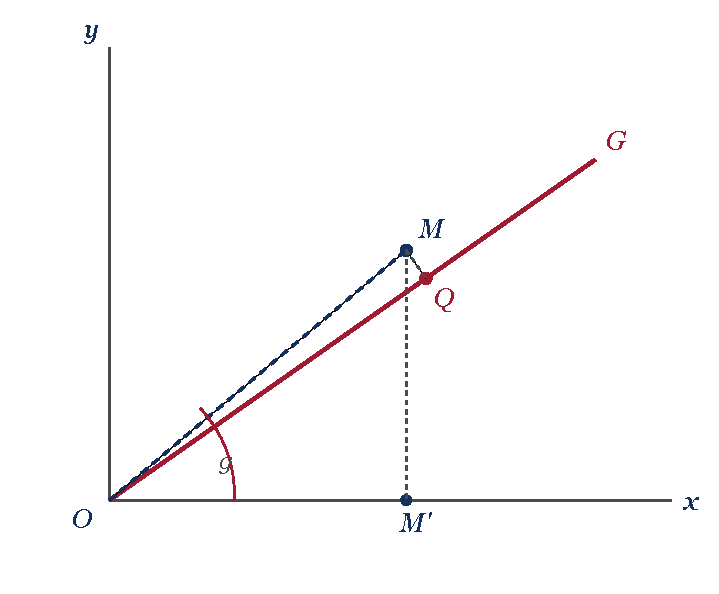
\includegraphics[width=0.55\textwidth]{figuras/pdf/cap02-fig1.pdf}
\caption{Descomposición de la vibración $OM$ en la dirección $OG$ del
polarizador $\Pi''$: $OQ$ es la componente que sobrevive, $MQ$ la que se
destruye.}
\label{fig:cap2-1}
\end{figure}

Para obtener la intensidad luminosa en un punto $P$, buscaremos el valor
medio de $OQ^2$ para un número muy grande de vibraciones. El valor medio
de esta cantidad durante una vibración es
\[
\frac{1}{2}\Bigl[A_0^2\cos^2g+B_0'^2\sin^2g
+2A_0B_0'\sin g\cos g\cos(\theta+\psi)\Bigr].
\]

Si, antes de su paso por los polarizadores $\Pi$ y $\Pi'$, la luz era
natural, $\theta$ puede tomar una infinidad de valores, y en el valor
medio de la expresión anterior el término rectángulo que contiene
$\cos(\theta+\psi)$ desaparece. En este caso no hay interferencia.

Cuando, por el contrario, la luz está polarizada rectilíneamente antes de
su paso por los polarizadores $\Pi$ y $\Pi'$, la cantidad $\theta$ es
igual a $0$ o a $\pi$. El valor del término rectángulo es, salvo el
signo,
\[
2A_0B_0'\cos g\sin g\cos\psi;
\]
su valor medio durante un gran número de vibraciones contendrá
$\cos\psi$, y los rayos interferirán.
